%
% File naaclhlt2016.tex
%

\documentclass[11pt,letterpaper]{article}
\usepackage{naaclhlt2016}
% \usepackage[textsize=tiny]{todonotes}
\usepackage{times}
\usepackage{latexsym}
\usepackage{graphicx}
\usepackage{lipsum}
\usepackage{url}
\usepackage{array}
\usepackage{lmodern}
\usepackage{siunitx}
\usepackage{booktabs}
\usepackage{etoolbox}
% New command for horizontal alignment in tables (P instead of p):
\newcolumntype{P}[1]{>{\centering\arraybackslash}p{#1}}
% New command for making text bold in tables (\B):
\sisetup{detect-weight,mode=text}
\renewrobustcmd{\bfseries}{\fontseries{b}\selectfont}
\renewrobustcmd{\boldmath}{}
\newrobustcmd{\B}{\bfseries}
% Coloring text in table
\usepackage{xcolor}
\usepackage{color}
\usepackage[normalem]{ulem} % for striking out text (for commenting process) using \sout

%\naaclfinalcopy % Uncomment this line for the final submission
\def\naaclpaperid{***} %  Enter the naacl Paper ID here

% To expand the titlebox for more authors, uncomment
% below and set accordingly.
% \addtolength\titlebox{.5in}    

\newcommand\BibTeX{B{\sc ib}\TeX}
% \newcommand{\marco}[1]{\todo[color=green!40]{MB: #1}}
% \newcommand{\dieuwke}[1]{\todo[color=red!40]{DH: #1}}
\newcommand{\dieuwke}[1]{\textcolor{red}{(DH: #1)}}
% \newcommand{\yair}[1]{\todo[color=blue!40]{YL: #1}}
% \newcommand{\german}[1]{\todo[color=purple!40]{GK: #1}}

\title{The emergence of number and syntax units in LSTM language models}

% Author information can be set in various styles:
% For several authors from the same institution:
% \author{Author 1 \and ... \and Author n \\
%         Address line \\ ... \\ Address line}
% if the names do not fit well on one line use
%         Author 1 \\ {\bf Author 2} \\ ... \\ {\bf Author n} \\
% For authors from different institutions:
% \author{Author 1 \\ Address line \\  ... \\ Address line
%         \And  ... \And
%         Author n \\ Address line \\ ... \\ Address line}
% To start a seperate ``row'' of authors use \AND, as in
% \author{Author 1 \\ Address line \\  ... \\ Address line
%         \AND
%         Author 2 \\ Address line \\ ... \\ Address line \And
%         Author 3 \\ Address line \\ ... \\ Address line}
% If the title and author information does not fit in the area allocated,
% place \setlength\titlebox{<new height>} right after
% at the top, where <new height> can be something larger than 2.25in
\author{Author 1\\
	    XYZ Company\\
	    111 Anywhere Street\\
	    Mytown, NY 10000, USA\\
	    {\tt author1@xyz.org}
	  \And
	Author 2\\
  	ABC University\\
  	900 Main Street\\
  	Ourcity, PQ, Canada A1A 1T2\\
  {\tt author2@abc.ca}}

\date{}

\begin{document}

\maketitle

% Abstract
\begin{abstract}
  Recent work has shown that LSTMs trained on a generic language modeling objective capture syntax-sensitive generalizations such as long-distance number agreement. 
  We have however no mechanistic understanding of how they accomplish this remarkable feature, and some have conjectured it depends on heuristics that do not truly
  take hierarchical structure into account. 
  We present here a detailed study of the inner mechanics of number tracking in LSTMs at the single neuron level. 
  We discover that number information is managed by very few ``grandmother cells'' in a localist fashion. 
  Importantly, the behaviour of the number cells is partially controlled by other units that are independently shown to track the syntactic structure of sentences. 
  We conclude that LSTMs are, to some extent, implementing genuinely syntactic processing mechanisms, paving the way to a more general understanding of grammatical encoding in LSTMs.
\end{abstract}


% Sections
\section{Introduction}

In the last years, recurrent neural networks (RNNs), and particularly
long-short-term-memory (LSTM) architectures
\cite{Hochreiter:Schmidhuber:1997}, have been successfully applied to
a variety of NLP tasks. This has spurred interest in whether these
generic sequence-processing devices are discovering genuine structural
properties of language in their training data, or whether their
success can be explained by opportunistic surface-pattern-based
heuristics.

Until now, this debate has mostly relied on ``behavioural'' evidence:
The LSTM is treated as a black box, and its capacities are indirectly
inferred by its performance on linguistic tasks. We take here a
complementary ``neuroscientific'' approach: We thoroughly investigate
the inner dynamics of an LSTM performing the number agreement task,
striving to achieve a mechanistic understanding of how it accomplishes
it. We find that the LSTM specialized very few ``grandma'' cells
\cite{Bowers:2009} to carry number features from the subject to the
verb across the intervening material. Interestingly, the LSTM also
possesses a more distributed mechanism to predict number when subject
and verb are close, with the grandma number cells only playing a
crucial role in more difficult long-distance cases. Crucially, we
independently identified a set of cells tracking syntactic structure,
and found that one of them encodes the presence of an embedded phrase
separating the main subject-verb dependency, and has strong efferent
connections to the long-distance number cells, suggesting that the
network relies on genuine syntactic information to regulate
agreement-feature percolation.

Our analysis thus provides direct evidence for the claim that LSTMs
trained with language modeling on unannotated corpus data, despite
lacking significant linguistic priors, learn to perform
structure-dependent linguistic operations. In turn, this suggests that
raw linguistic input and generic memory mechanisms, such as those
implemented in LSTMs, may suffice to trigger the induction of
non-trivial grammatical rules.

%\yair{In case we would need further compression in the intro, we could consider omitting the penultimate paragraph that describes the results, and leave the reader with only the teaser in the current last paragraph.}


%\marco{Yair, I think your intro is excellent, but I feel is too long for a NAACL conference paper, where probably even mine will have to be shortened: I'd comment it out and keep it for the journal version.}

%\yair{I love the intro as is. We could perhaps try to anchor the work within a slightly wider context though, by first discussing the debate between structure-based vs. statistical/heuristic approachs to sentence processing in humans in both linguistics and neuroscience. Then, describing the recent findings about LSTM-LMs as a parallel debate about RNNs, and finally to stress the advantages of working out the latter debate about LSTM-LM through computational simulations, like our work, in contributing to insights regarding the original debate in humans. I therefore sketched a possible intro paragraph, but we could postpone this for the more 'cognitive' audience in the longer version (and perhaps its also anyway too ambitious to describe our work as contributing in any way to the classic debate).}

%\yair{Sentence comprehension requires to process dependencies between words in the sentence. Such dependencies may affect the meaning ascribed to sentence constituents and the prediction of next ones. Two opposing theoretical approches have been suggested for sentence comprehension. The first, more traditional one, suggests that structure-based syntactic processes are the principal computational capacity of human language (cite Chomsky 57,72; Pinker 95; Hauser et al 2002). According to this approach, word dependencies are described by syntactic trees and their processing is described by structure-based parsing computations (cite). The second, more recent approach, suggests that more fuzzy processes may underline human-language computations, thus embrasing 'good enough parsing' and canny heuristics (cite, eg, Traxler 2014; Ferreira, F., \& Patson, N. D. 2007; ). According to this approach, word dependencies, and sentence comprehension in general, are instead desribed by information-based and Bayesian theories (e.g., Levy R, 2009; Gibson et al 2013). Following this, a parallel debate has emerged in the neuroscientific community, drawing into consideration also the continuous dyanmics of biological nerual network akin to fuzzy computations. On the one hand, several studies provided evidence that brain processes lend themselves to interpreations from traditional syntax theories (cite Friederici, 2006, 2013, Nelson 2017). On the other hand, other studies have provided evidence against the primacy of such syntactic and structure-based computations in neural processing of sentences (e.g., Fedorenko 2018). Interestingly, recently, a similar debate about sentence processing has emerged about state-of-the-art sequential-learning models in the field of artificial neural networks (eg Linzen et al 2016, Gulordava:etal:2018, Kuncoro:etal:2018b, Linzen:Leonard:2018; see also Lake B et al:Behav and Brain sci:2017 for a related, more general, scope of debate, awakening an older one fodor\&pylyshyn:1988). Since both artifical and biological neural networks preserve the tension between their continuous dynamics and the discrete, structure-based, character of syntacic processing, while ANNs provide flexibility in conducting experiments, also going through tremendous recent advances, looking into this debate from this perspective may turn out to be in particular instructional.}



\section{Related work}

Starting with the seminal work of \newcite{Linzen:etal:2016},
long-distance number agreement (``the \textbf{boy} near the cars
\textbf{greets}\ldots'') has emerged as a standard way to probe the
syntactic capabilities of RNNs. Following
mixed initial results by Linzen and colleagues and
\newcite{Bernardy:Lappin:2017}, \newcite{Gulordava:etal:2018} and
\newcite{Kuncoro:etal:2018a} have robustly established that LSTMs
trained with a language modeling objective on raw data achieve
near-human performance on the agreement task. While Gulordava and
colleagues provided some evidence that the LSTMs are relying on
genuine syntactic generalizations, \newcite{Kuncoro:etal:2018b} and
\newcite{Linzen:Leonard:2018} suggested that the LSTM achievements
can, at least in part, be accounted by superficial heuristics (e.g., ``percolate the number of the first noun in a sentence''). Other
recent work has extended syntax probing to other phenomena such as
negative polarity items and island constraints
\cite{Chowdhury:Zamparelli:2018,jumelet2018language,marvin2018targeted,wilcox2018rnn}.

While \newcite{Linzen:etal:2016} presented intriguing qualitative data
showing cells that track grammatical number in a network directly trained on
the agreement task, most of the following work focused on testing the
network output behaviour, rather than on understanding how the latter
follows from the inner representations of the network. Another research line
studied linguistic processing in neural networks through `diagnostic classifiers', that is, classifiers trained to
predict a certain property from network activations
\cite[e.g.,][]{gelderloos2016phonemes,Adi:etal:2017,alain2017understanding,Hupkes:etal:2017}. This approach may give insight into which information is encoded by the
network in different layers or at different time points, but it only
provides indirect evidence about the specific mechanics of linguistic
processing in the network.

Other studies are closer to our approach in that they attempt to
attribute function to specific network cells, often by means of
visualization
\cite{Karpathy:etal:2016,li2016visualizing,tang2017memory}. \newcite{Radford:etal:2017},
for example, detected a ``sentiment'' grandmother cell in a
language-model-trained network.  \newcite{Kementchedjhieva:Lopez:2018}
recently found a character-level RNN to track morpheme boundaries in a
single cell. We are however not aware of others studies systematically
characterizing the processing of a linguistic phenomenon at the level of
RNN cell dynamics, as is the attempt in the study hereby presented.
\section{Data}
\subsection{Number-agreement tasks}

\begin{table}[tb]
  \centering
  \begin{footnotesize}
  \begin{tabular}{l@{\hskip1pt}l}
    \B Simple & the boy greets the guy\\
    \B Adv & the boy probably greets the guy\\
    \B 2Adv & the boy most probably greets the guy\\
    \B CoAdv &  the boy openly and deliberately greets the guy\\
    \B NamePP & the boy near Pat greets the guy\\
    \B NounPP & the boy near the car greets the guy\\
    \B SubjRel & the boy that avoids the girl greets the guy\\
    \B ObjRel  & the boy that the girl avoids greets the guy \\
    \B ObjRel0 &  the boy the girl avoids greets the guy\\
  \end{tabular}
  \end{footnotesize}
  \caption{NA tasks illustrated by representative
    singular sentences.}
  \label{tab:data-sets}
\end{table}

We generated number-agreement tasks (NA-tasks) with fixed syntactic
structures and varied lexical material that probe subject-verb number
agreement in increasingly challenging setups. The different structures
are illustrated in Table \ref{tab:data-sets} by examples where all
forms are in the singular. Distinct sentences were randomly generated
by selecting (different) words from pools of 20 subject/object nouns,
15 verbs, 10 adverbs, 5 prepositions, 10 proper nouns and 10 location
nouns. The items were selected so that their combination would not
lead to semantic anomalies.For each NA-task, we generated singular and
plural versions of each sentence. We refer to each such version as a
\textit{condition}. For NA-tasks that have other nouns occurring between
subject and main verb, we also systematically varied their number,
resulting in four conditions. For example, the NounPP sentence in the
table illustrates the SS (singular-singular) condition. The
corresponding sentences in the other conditions are: ``the boy near
the cars greets the guy'' (SP), ``the boys near the car greet the
guy'' (PS), and ``the boys near the cars greet the guy'' (PP).


\textcolor{red}{Possibly move this to Models or Results section.} For
each NA-task, model performance was evaluated for each of its
conditions separately, by computing its accuracy in predicting the
correct form of the main verb. Specifically, for each sentence from a
condition, the model was presented with all words up to the one
immediately preceding the main verb. If the model assigned higher
likelihood to the correct form of the verb than to its counterpart
with the wrong number, then the trial was marked as a hit.

\textcolor{red}{Yair: consider move these explanations about contrasts to the results section:} \sout{Note that 2Adv features the same subject-verb
distance as NamePP, but without gender-carrying words acting as
possible distractors in the middle. Similarly, CoAdv can serve as a
distractor-free control for NounPP.}

Task sata-set sizes across conditions ranged from 600 (Simple) to 18k sentences (relatives),
based on the possibilities for variation allowed by the combinatorics
given each structure.\footnote{We uploaded the data-set generation
  script as supplementary material.}

Finally, we also used the naturalistic, corpus-derived agreement test set of \newcite{Linzen:etal:2016}, in the version made available by \newcite{Gulordava:etal:2018}.

\subsection{Number of open nodes}


% \subsection{Synthetic data}

% \subsubsection{Stimuli for the number-agreement task (NA-task)}
% This section describes the generation process of synthetic sentence stimuli for the number-agreement task (NA-task). 
% These sets of stimuli were used to evaluate the performance of both full- and ablated models on the NA-task. 

% Each NA-task contained sentences with a fixed syntactic structure, such as ``Det Noun Adv Verb'' or ``Det Noun P Det Noun Verb'', and each task was composed of several \textit{conditions} depending on the possible assignments of grammatical number to the nonu(s) in the sentence. 
% For example, one NA-task contained sentences of the form: ``Det Noun Verb'', and had two conditions corresponding to the two possible number values of its noun. 
% So the first conditiond such as ``The boy runs'', and the ablated network was tested on predicting the correct verb form. 
% This task had two conditions, corresponding to the two possible assignments of grammatical number (singular or plural) to the main noun. 
% Another NA-task contained sentences of the form: ``Det Noun-1 P Det Noun-1 Verb'', such as ``The boy behind the girls jumps''. 
% This task had four conditions, corresponding to the four possible assignments of grammatical number to noun-1 and noun-2.

% The network was evaluated on predicting the correct verb form (singular or plural).

% \subsection{Corpus data}

% \textcolor{gray}{\lipsum[1]}


\section{The models}

The recurrent models that are the focus of our studies are long short term memory models \cite[LSTMs]{Hochreiter:Schmidhuber:1997}.
To inspect the internal dynamics of these models, we use additional linear models to extract information from the hidden state of trained language models.
In this section, we describe the language model we study (\ref{ssec:lstm_lm}) as well as the meta models we use to analyse the hidden states of this language model (\ref{ssec:dc}).

\subsection{LSTM language model}\label{ssec:lstm_lm}

\paragraph{Model description} We consider the pretrained LSTM LM that was made available by \cite{Gulordava:etal:2018}.\footnote{We report our results only for this model, but acertained the robustness of these results by repeating the tests for models trained with different seeds and drop-out values}
This model has two LSTM layers with 650 dimensions, an output layer with vocabulary size 50000 and an embedding layer of 650 dimensions.
In our experiments, we investigate the different components of both layers of the LSTM, given by the equations below:
\begin{align}
    h_t & = o_t\circ \tanh(c_t)\\ 
     c_t & = f_t\circ c_{t-1} + i_t\circ \widetilde{c}_t\\
     \widetilde{c}_t & = \tanh(W_cx_t + U_ch_{t-1} + b_c)\\
     f_t & = \sigma(W_fx_t + U_fh_{t-1} + b_f) \\
     i_t & = \sigma(W_ix_t + U_ih_{t-1} + b_i) \\
     o_t & = \sigma(W_ox_t + U_oh_{t-1} + b_o)
\end{align}

We will refer to the n$^{th}$ unit in the first and second layer with the terms \unit{1}{n} and \unit{2}{n}, respectively.

\paragraph{Model evaluation on NA-tasks}
Model performance was evaluated on each NA-task and conditions by computing its accuracy in predicting the correct form of the main verb. Specifically, for each sentence, the model was presented with all words up to the one immediately preceding the main verb. If the model assigned higher likelihood to the correct form of the verb than to its counterpart with the wrong number then the trial was marked as a hit. Model accuracy was then computed by counting the fraction of hits across the entire set of sentences in the condition, and is denoted in what follows as ACC$_{NA-task, condition}$.


\subsection{Regression model}\label{ssec:dc}

To understand which information is encoded in the hidden states and gates of the LSTM language model, we use a technique that is commonly used in neuroscience (ref?) but has recently also gained traction in the field of computational linguistics: training an additional model to predict information from these hidden states and gates \cite{Adi:etal:2017,Hupkes:etal:2017}.  

In our case, we aim to assess if the internal states of our language model incode information about the \textit{syntactic depth} of the sentence it is processing.
The setup is as follows.

- Explain that the model was used to predict the depth of the syntactic tree from network activity
\paragraph{Model description}
- Describe the Features: network activity (hidden/cell activity)
- Describe the label: Tree depth (\ref{ssec:n_opennodes})
- Describe the model: A Ridge/LASSO model.
- Describe{Model training and evalution}
- Model training: nested 5-fold CV procedure. Train/val/test. Optimal regularization size was estimated from the validation set (report optimal lamda - figures in FAIRNS.pdf on slack)
- model evaluation: R-squared on test set. Report resulting values (text+figures in FAIRNS.pdf). 





% Results
\section{Experiments}\label{sec:results}
To successfully perform the NA-task, the LSTM should: (1) encode and store the grammatical number of the subject; and (2) track the main subject-verb syntactic dependency. The latter information is important for identifying the time period during which the network should store the subject number, and when it should output it and allow to update number information. This section describes the `neural circuit' that encodes and processes this information in the LSTM.

\begin{center}
\begin{table}[ht]
\centering
\begin{tabular}{|P{2.3cm}|P{0.4cm}||P{0.6cm}|P{0.6cm}|P{0.6cm}|}
\hline
    \B \multirow{2}{*}{NA task} & \B \multirow{2}{*}{C} & \multicolumn{2}{c|}{\B Ablated}& \multirow{2}{*}{\B Full} \\
    \cline{3-4}
    & & \B \textbf{\unit{2}{126}} & \B \textbf{\unit{2}{338}} & \\
\hline

% Singular conditions
Simple & S & - &  - &  \textcolor{red}{100} \\

Adv & S & - &  - &  \textcolor{red}{100} \\

2Adv & S & - &  - &  \textcolor{red}{99.9} \\

CoAdv & S & - &  \textcolor{red}{82} &  \textcolor{red}{98.7} \\

namePP & SS & - &  - &  \textcolor{red}{99.3} \\

nounPP & SS & - &  - &  \textcolor{red}{99.2} \\

nounPP & SP &  - &  \textcolor{red}{54.2} &  \textcolor{red}{87.2} \\

nounPPAdv & SS &  - &  - & \textcolor{red}{99.5} \\

nounPPAdv & SP &  - &  \textcolor{red}{54.0} & \textcolor{red}{91.2} \\


\hline
% Plural conditions
Simple & P &  - &  - &  \textcolor{blue}{100} \\

Adv & P &  - &  - &  \textcolor{blue}{99.6} \\

2Adv & P & - &  - &   \textcolor{blue}{99.3} \\

CoAdv & P &  \textcolor{blue}{79.2} &  - &   \textcolor{blue}{99.3} \\

namePP & PS & \textcolor{blue}{39.9} &  - &   \textcolor{blue}{68.9} \\

nounPP & PS &  \textcolor{blue}{48.0} & - &   \textcolor{blue}{92.0} \\

nounPP & PP &  \textcolor{blue}{78.3} & - &   \textcolor{blue}{99.0} \\

nounPPAdv & PS & \textcolor{blue}{63.7} &  - &   \textcolor{blue}{99.2} \\

nounPPAdv & PP & - &  - &   \textcolor{blue}{99.8} \\

\hline

\B Linzen & \B - &   75.3 &  - &  93.9 \\
\hline

\end{tabular}
% \tiny
\caption{Ablation-experiments results: Percentage accuracy in all NA-tasks. Full: non-ablated model, C: condition, S: singular, P: plural. Red: Singular subject, Blue: Plural subject. Performance reduction less than 10\% is denoted by `-'.  \label{tab:ablation-results}}
\end{table}
\end{center}

\begin{figure*}[ht]
    \centering
    \begin{subfigure}{\textwidth}
            \centering
            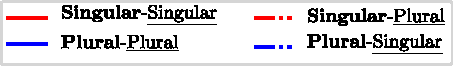
\includegraphics[width=0.3\linewidth]{Figures/legend.pdf}
    \end{subfigure}
    \bigskip
    \begin{subfigure}{0.32\textwidth}
            \centering
            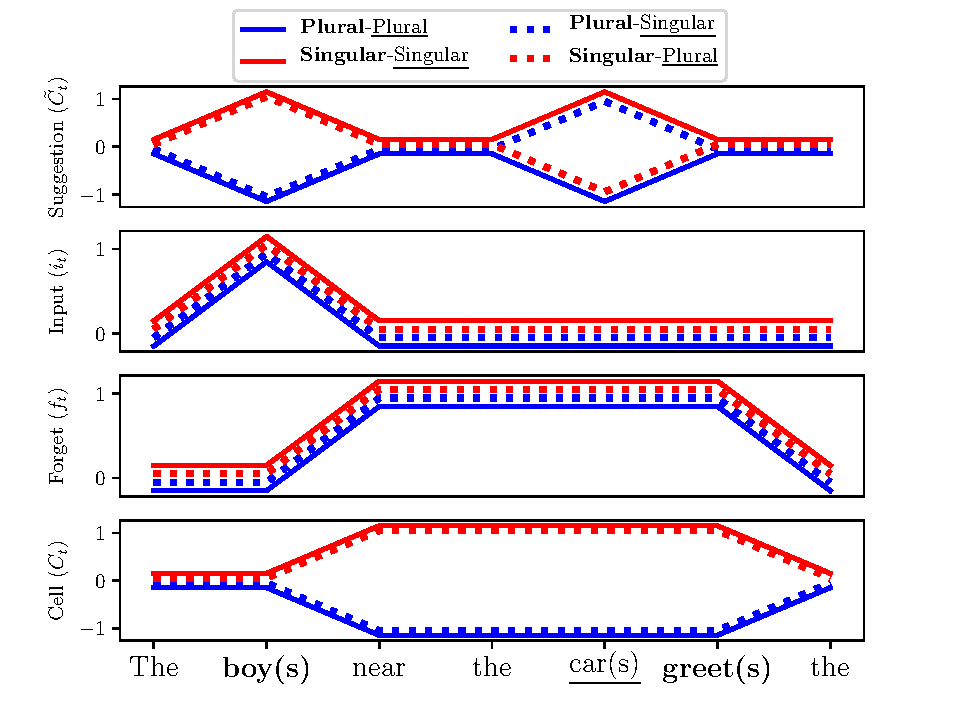
\includegraphics[width=\linewidth]{Figures/unit-timeseries-cartoon.pdf}
            \subcaption{Prediction (singular)}
    \label{fig:cartoon}
    \end{subfigure}
    \begin{subfigure}{0.32\textwidth}
            \centering
            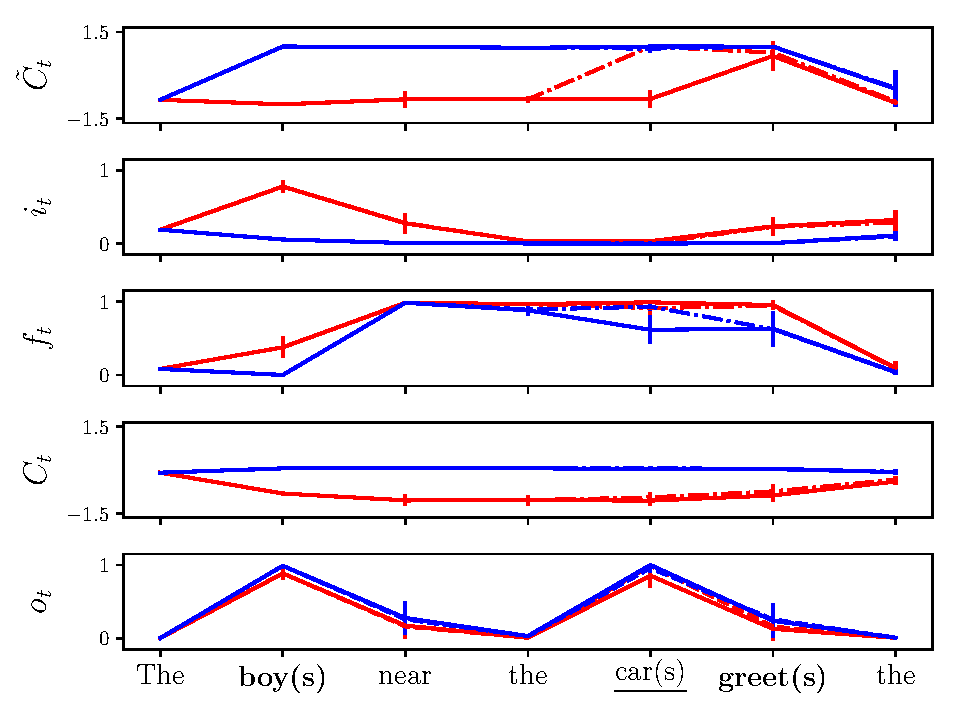
\includegraphics[width=\linewidth]{Figures/nounpp_987.pdf}
            \subcaption{\unit{2}{338} (singular)}
    \label{fig:singular-unit}
    \end{subfigure}
    \begin{subfigure}{0.32\textwidth}
            \centering
            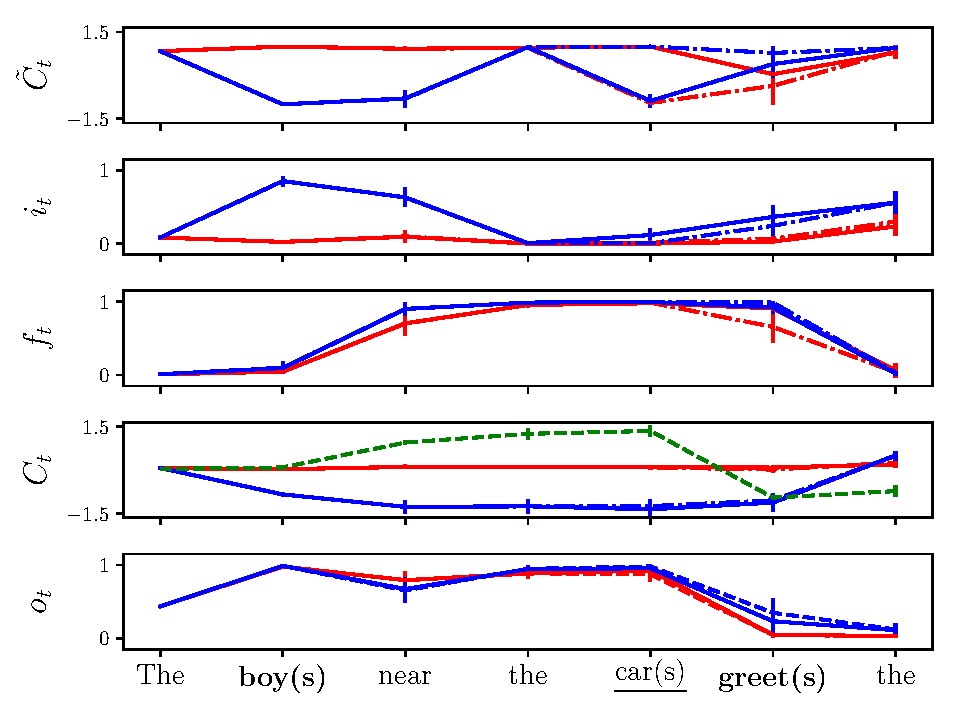
\includegraphics[width=\linewidth]{Figures/nounpp_775.pdf}
            \subcaption{\unit{2}{126} (plural)}
    \label{fig:plural-unit}
    \end{subfigure}
\caption{Cell and gate activations during processing of sentences with a prepositional phrase between subject and verb. Values in (b) and (c) are averaged across all condition sentences, with error bars showing standard deviations.}
\end{figure*}

\subsection{Long-range number units}\label{subsec:ablation}
We first tested LSTM performance on Linzen's data and on the NA-tasks of Table
\ref{tab:data-sets}. Following
\newcite{Linzen:etal:2016} and later work, we computed the likelihood
that the LSTM assigns to the main verb of each sentence given the
preceding context, and compared it to the likelihood it assigns to the
wrong verb inflection. Accuracy in a given condition was measured as the proportion of sentences in the condition where the model assigned a higher likelihood to the correct form than to the wrong one.

Network performance is reported in Table \ref{tab:ablation-results}
(right column -- `Full'). First, results show that some NA-tasks and
conditions are more difficult than others. For example, performance on
the Simple (0-distance) NA-task is better than that on the Co-Adv
NA-task, which in turn is better than that of the nounPP
tasks. Second, as expected, incongruent conditions (the
number-mismatch conditions of namePP, nounPP and nounPPAdv) reduce
network performance. Third, for long-range dependencies, reliably
encoding singular subject across an interfering noun is more difficult
than a plural subject: for both nounPP and nounPPAdv, PS is easier
than SP. A possible explanation for this finding is that in English the plural form is
almost always more frequent than the singular one, as the latter only
marks third person singular, whereas the former is identical to the
infinitive and other forms. Thus, if the network reverts to unigram
probabilities, it will tend to prefer the plural. Last, we replicated
the results of \newcite{Gulordava:etal:2018} for the Linzen NA-task.

\paragraph{Looking for number units through ablation} Number
information may be stored in the network in either a local, sparse, or
a distributed way, depending on the fraction of active units that
carry it.  We hypothesized that if the network uses a local or sparse
coding, meaning that there's a small set of units that encode number
information, then ablating these units would lead to a drastic
decrease in performance in the NA-tasks.  To test this, we ablated
each unit of the network one at a time, by fixing its activation to zero,
and tested on the tasks.

Two units were found to have exceptional effect on network performance
(Table \ref{tab:ablation-results}, \unit{2}{126} and \unit{2}{338}
columns).\footnote{Units 1-650 belong to the first layer, 651-1300 to
  the second. All units detected by our analyses come from the latter.} Ablating them reduced network performance by more than 10\%
across various conditions, and importantly, they were the only units
whose ablation consistently brought network performance to around
chance level in the more difficult incongruent conditions of the
namePP, nounPP and nounPPAdv
tasks. 

Moreover, the ablation effect depended on the grammatical number of the subject: ablating \unit{2}{126} significantly reduces
network performance only if the subject is plural (P, PS or PP conditions) and \unit{2}{338}
only if the subject is singular (S, SP or SS conditions). In what follows, we will therefore
refer to these units as the `plural' and `singular' units, respectively,
or long-range (LR) number units when referring to both. Finally, we note that although the Linzen NA-task contained mixed stimuli from many types of conditions, the plural unit was found to have a substantial effect on average on network performance. The singular unit didn't show a similar effect in this case, which highlights the importance of using carefully crafted stimuli, as in the nounPP and nounPPAdv tasks, for understanding network dynamics. Taken
together, these results suggest a highly local coding scheme of
grammatical number when processing long-range dependencies.

\paragraph{Visualizing gate and cell-state dynamics}\label{subsec:gate-dynamics}
To understand the functioning of the number units, we now look
into their gate and state dynamics during sentence processing. We
focus on the nounPP NA-task, which is the simplest NA-task including a
long-range dependency having an interfering noun in both SP and PS
incongruent conditions.

Recall the standard LSTM memory update and output rules \cite{Hochreiter:Schmidhuber:1997}:
\begin{align} 
    C_t &= f_t\circ C_{t-1} + i_t\circ \widetilde{C}_t \label{eq:update-rule} \\
     h_t &= o_t\circ \tanh(C_t) \label{eq:output},
\end{align}
where $f_t, i_t, o_t \in (0,1)$ are gating scalars computed by the network, and $\widetilde{C}_t \in (-1, 1)$ is an update candidate for cell value.

Consider now how a number unit may reliably encode and store subject
number across interfering nouns.  Figure\ref{fig:cartoon} exemplifies
this for a singular unit, showing the desired gate and cell
dynamics. The four conditions are represented with separated curves -
red for singular subject, blue for plural, and dashed lines for
incongruent conditions. Gate and cell activity at time points
unrelated to solving the NA-task are masked with white, as we do not
make precise predictions for them.

The update rule of the LSTM cell has two terms
(Eq.~\ref{eq:update-rule}).\footnote{We abuse notation here, using the
  symbols denoting whole layers in equations (\ref{eq:update-rule}) and
  (\ref{eq:output}) to denote the components of single cells.} In the
first, $f_t \circ{} C_{t-1}$, the forget gate controls whether to keep
the previous cell content ($f_t=1$: perfect remembering) or forget it
($f_t=0$: complete forgetting). In the second,
$i_t\circ{} \tilde{C}_t$, the input gate controls whether the
information currently presented to the network, as encoded by
$\tilde{C}_t$, should be written onto the cell ($i_t=1$: full access)
or not ($i_t=0$). The singular unit can thus use these gates to
reliably store number information across long-range
dependencies. Specifically, the unit can (enumeration follows the same order as the panels in Figure~\ref{fig:cartoon}): (1) encode subject
number via $\tilde{C}_{t_{subject}}$ with different values for
singular and plural; (2) open the input gate \textit{only} when a
singular subject is presented ($i_{t_{subject}} = 1$ in red curves \textit{only}) and protect it from interfering nouns ($i_t=0, t_{subject}<t<t_{verb}$); (3) at the same time,
clear the cell from previously stored information
($f_{t_{subject}}=0$) and then store subject number across the entire
dependency ($f_t=1, t_{subject}<t<t_{verb}$); (4) this will result in
stable encoding of subject number in the cell $C_t$ throughout the
dependency; (5) finally, output subject number at the right moment,
when predicting the verb form ($o_{t_{verb}-1}=1$)
(Eq.~\ref{eq:output}).

Figures \ref{fig:singular-unit} and \ref{fig:plural-unit} present the actual gate and cell dynamics of the singular and plural units. Both units follow the general solution for reliable number storage described above. Note that for $\tilde{C}_t$ and $i_t$, and as a result also for $C_t$, the plural unit `mirrors' the singular unit with respect to subject number (red curves of PP and PS vs. blue curves of SS and SP). This is in accordance with the results of the ablation experiments, which showed that ablating these units had an effect that depended on the grammatical number of the subject (Table \ref{tab:ablation-results}). This provides complementary support for the identification of these units as `singular' and `plural'.

A single divergence between the solution depicted in Figure \ref{fig:cartoon} and the actual dynamics of the number units is that input gate activity is smaller, but not zero, at the time step immediately following the subject. One speculative explanation is that this might be useful to process compound nouns. In these cases, subject number information is stored with the second noun, whereas in the case of simple nouns there is no `risk' of encountering an interfering noun immediately after the subject, making the delay in closing the gate safe.

\begin{figure}[b]
    \centering
    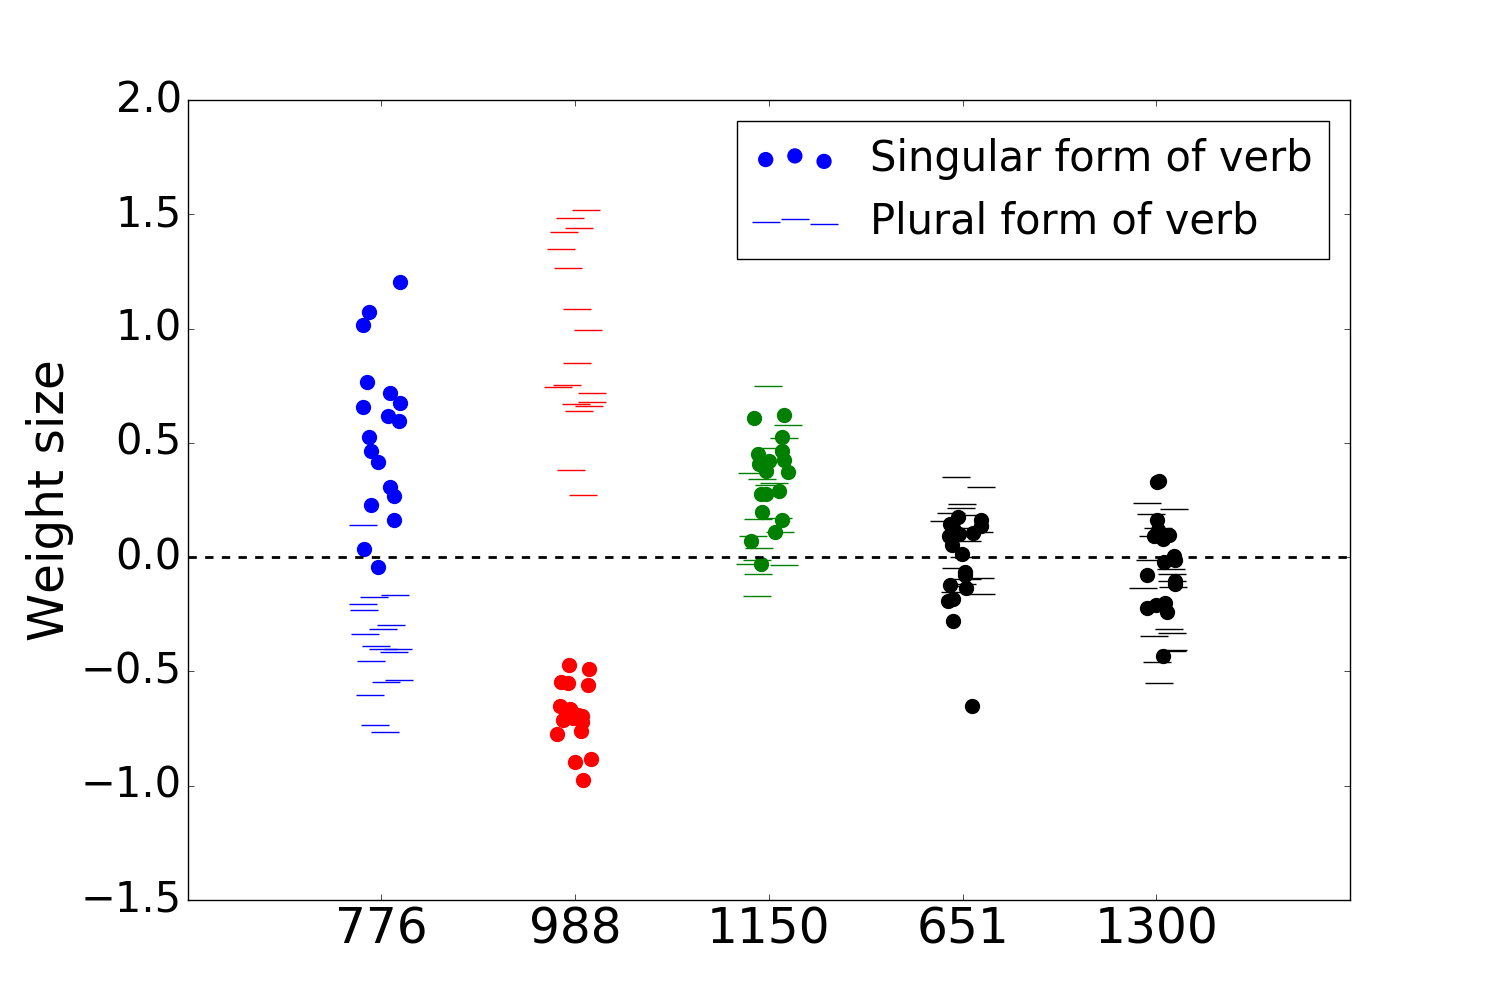
\includegraphics[height=4.6cm]{Figures/weight_dists_verbs.png}
    \caption{Efferent weights of the LR-units (\unit{2}{126} and \unit{2}{338}), the syntax unit (\unit{2}{500}; section \ref{sec:syntax-units}) and two arbitrary units (\unit{2}{1} and \unit{2}{650}).}
    \label{fig:output-weights}
\end{figure}

The singular and plural units had emerged at the second layer of the network. This seems appropriate if number information needs to be directly projected to the output layer for correct verb-form prediction. Moreover, number-unit output should be projected differently to singular and plural verb forms in the output layer, only increasing activity in output units representing the suitable form. For example, for the singular unit, since singular subjects are encoded with a negative value ($C_{t_{verb}-1}<-1$ in figure \ref{fig:singular-unit}), the more negative its efferent weights to singular verb forms in the output layer, the higher the probabilities of these verb forms would be. Figure \ref{fig:output-weights} shows the efferent weights of the LR-number units to all verbs in our data-sets. We found that, indeed, the efferent weights to the singular and plural verb forms are segregated from each other, with weight signs that correspond to the negative encoding of subject number used by both singular and plural units. Two other arbitrary units, \unit{2}{1} and \unit{2}{650}, and the syntax unit \unit{2}{500} to be described below (Section \ref{sec:syntax-units}) do not have segregated efferent weights to verb forms, as expected. 

\subsection{Short-range number information}
\begin{figure}
    \centering
    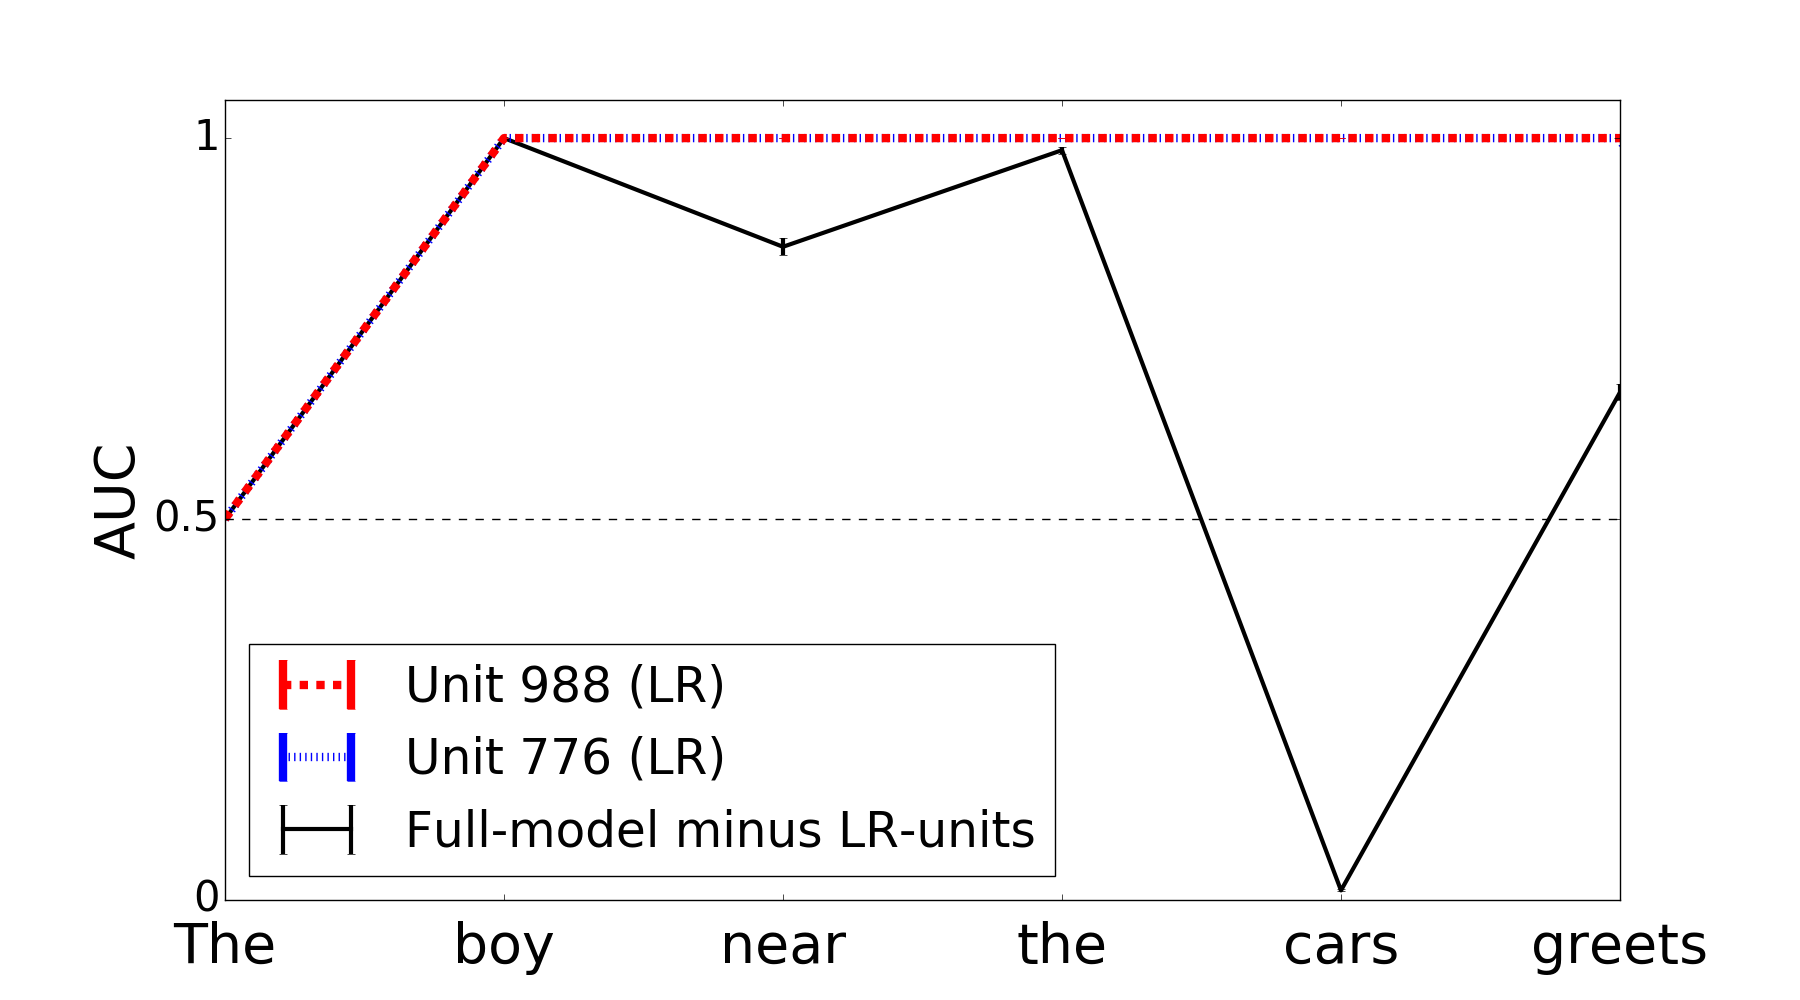
\includegraphics[height=4cm, width=8cm]{Figures/GAT1d_cell_.png}
    \caption{Generalization across time of subject-number prediction. Error bars represent standard deviations across cross-validation splits.}
    \label{fig:GAT}
\end{figure}

Performance on the easier NA-tasks (Simple, Adv, 2Adv) was not
impaired by single-unit ablations. This suggests that number may be
encoded also elsewhere in the network, perhaps via a more distributed
code. To verify this, we tested whether subject number can be decoded from the whole
pattern of activities in the network (excluding the two LR-number units)
and whether this decoding is stable across time \cite[see][for similar
observations and related methods]{Giulianelli:etal:2018}. We expected
this distributed activity network to track number in a
small time window after the subject, but, unlike the LR-number units,
to be affected by incongruent intervening nouns.

We trained a linear model to predict the grammatical number of the
subject from network activity in response to the presentation of the
subject, and tested its prediction on test sets from all time points
\cite{King:Dehaene:2014}, in incongruent conditions only of the nounPP
task. We used Area under of Curve (AUC) to evaluate model
performance. Figure \ref{fig:GAT} shows decoding across time of
subject number from cell activity of each number unit separately and
from cell activity of the entire network without these two units
(`Full model minus LR-units'). Results show that number information
can be efficiently decoded from other units in the network, and that
this information can be carried for several time steps (relatively
high AUC up to the second determiner). However, the way in which these
units encode number is sensitive to the last encountered noun, with
AUC decreasing to zero around the second noun (`cars'), whereas test
performance of the models trained on cell activity of the LR-number
units is consistently high. This confirms that number prediction is
supported both by the LR-number units, and by distributed activation
patterns of other short-range (SR) number units. The latter, however,
are not syntax-sensitive, and simply encode the number of the last
noun encountered.

%A full description of the SR-number units is beyond our scope. We
%tried however to identify specific SR-number units by training a
%linear model to predict subject number from single-unit activations,
%and by a careful inspection of the weights of a classifier trained on
%the full model (Figure \ref{fig:GAT}), accompanied by informal
%inspection of unit dynamics.

A full description of the SR-number units is beyond our scope. However, we note that 10 SR-number units in the second layer of the
network were identified, which had efferent weights with a similar segregated
structure as that of the LR units (Figure
\ref{fig:output-weights}). These units were indeed sensitive to the last
encountered noun: subject number could be decoded from single-unit cell activity
during its presentation (AUC$>0.9$), but activity `swaps' once an
interfering noun appears (i.e., AUC decreases to zero in a
generalization-across-time analysis). Finally, to validate the role of SR-number units in encoding number for easier NA-tasks, we ablated both SR and LR number
units (12 in total) or SR units only (10 in total) and evaluated network performance on these NA-tasks. Both experiments resulted in a significant reduction in task performance compared to 1,000 random equi-size ablations ($p<0.01$ in all `easier' tasks).

Intriguingly, we observed qualitatively that LR units are almost
always making the right prediction, even when the network predicts the
wrong number. The wrong outcome, in such cases, might be due to
interference from the syntax-insensitive SR units. We leave the study of LR-SR
unit interplay to future work.


\subsection{Syntax units}
\lipsum[1]

\subsubsection{Predicting syntactic-tree depth from network activity}
\lipsum[1]

\subsubsection{Ablation study}
\lipsum[1]

\subsection{Syntax-number units interactions}[t]
\lipsum[1]

\begin{figure*}
\centering
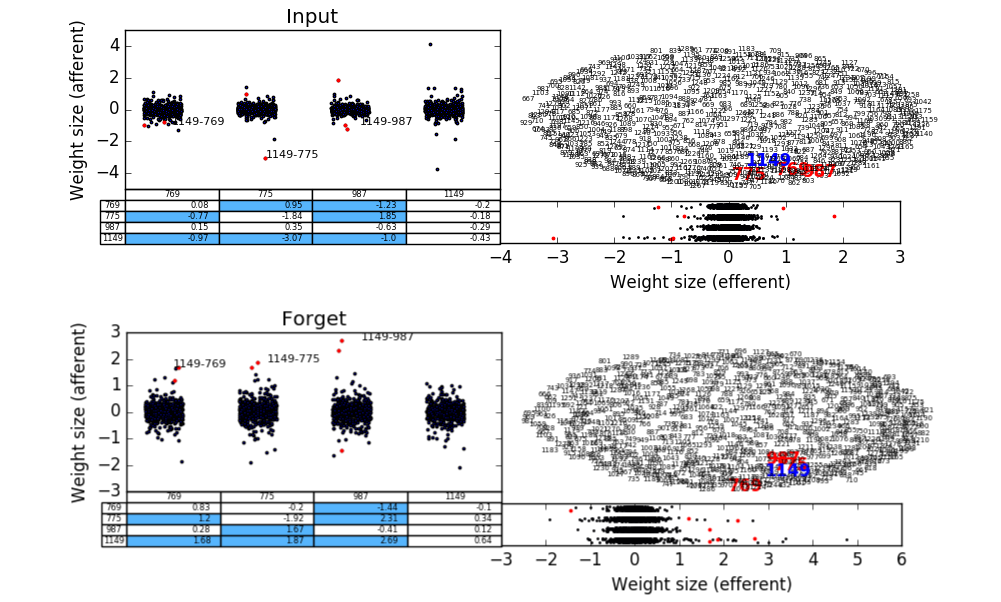
\includegraphics[width=\textwidth]{Papers_figures/Figure5_interactions.png}
\caption{Interaction among the syntax and number units. A value in the table represents the weight size from the unit appearing on the left to the unit appearing on the top row. (A) Distribution of all weight values to the unit appearing on the top row of the table. Outlier weights from the table (more than three standard-deviation above/below the mean) are marked in red; Weight values from the syntax to number units have in addition a corresponding text label. (B) Distribution of all weight values from the unit appearing on the left column of the table. Outlier weights are marked in red. (C)  A visualization of unit interactions. For each gate $g$, an interaction distance $d_{ij}^g$ between a pair of units $i$ and $j$ was first defined as: $d_{ij}^g=exp{-max{w_{ij}^g, w_{ji}^g}}$, where $w_{ij}^g$ is the weight from unit $j$ to the gate $g$ of unit $i$. Then, all interaction distances in the network were visualized using multidimensional scaling. Note that the interaction distances between the number units and between the syntax and number units are relatively close compared to the mean interaction distance in the network.}
\end{figure*}


\subsection{Processing of relative clauses}
\begin{figure*}[t]
\centering
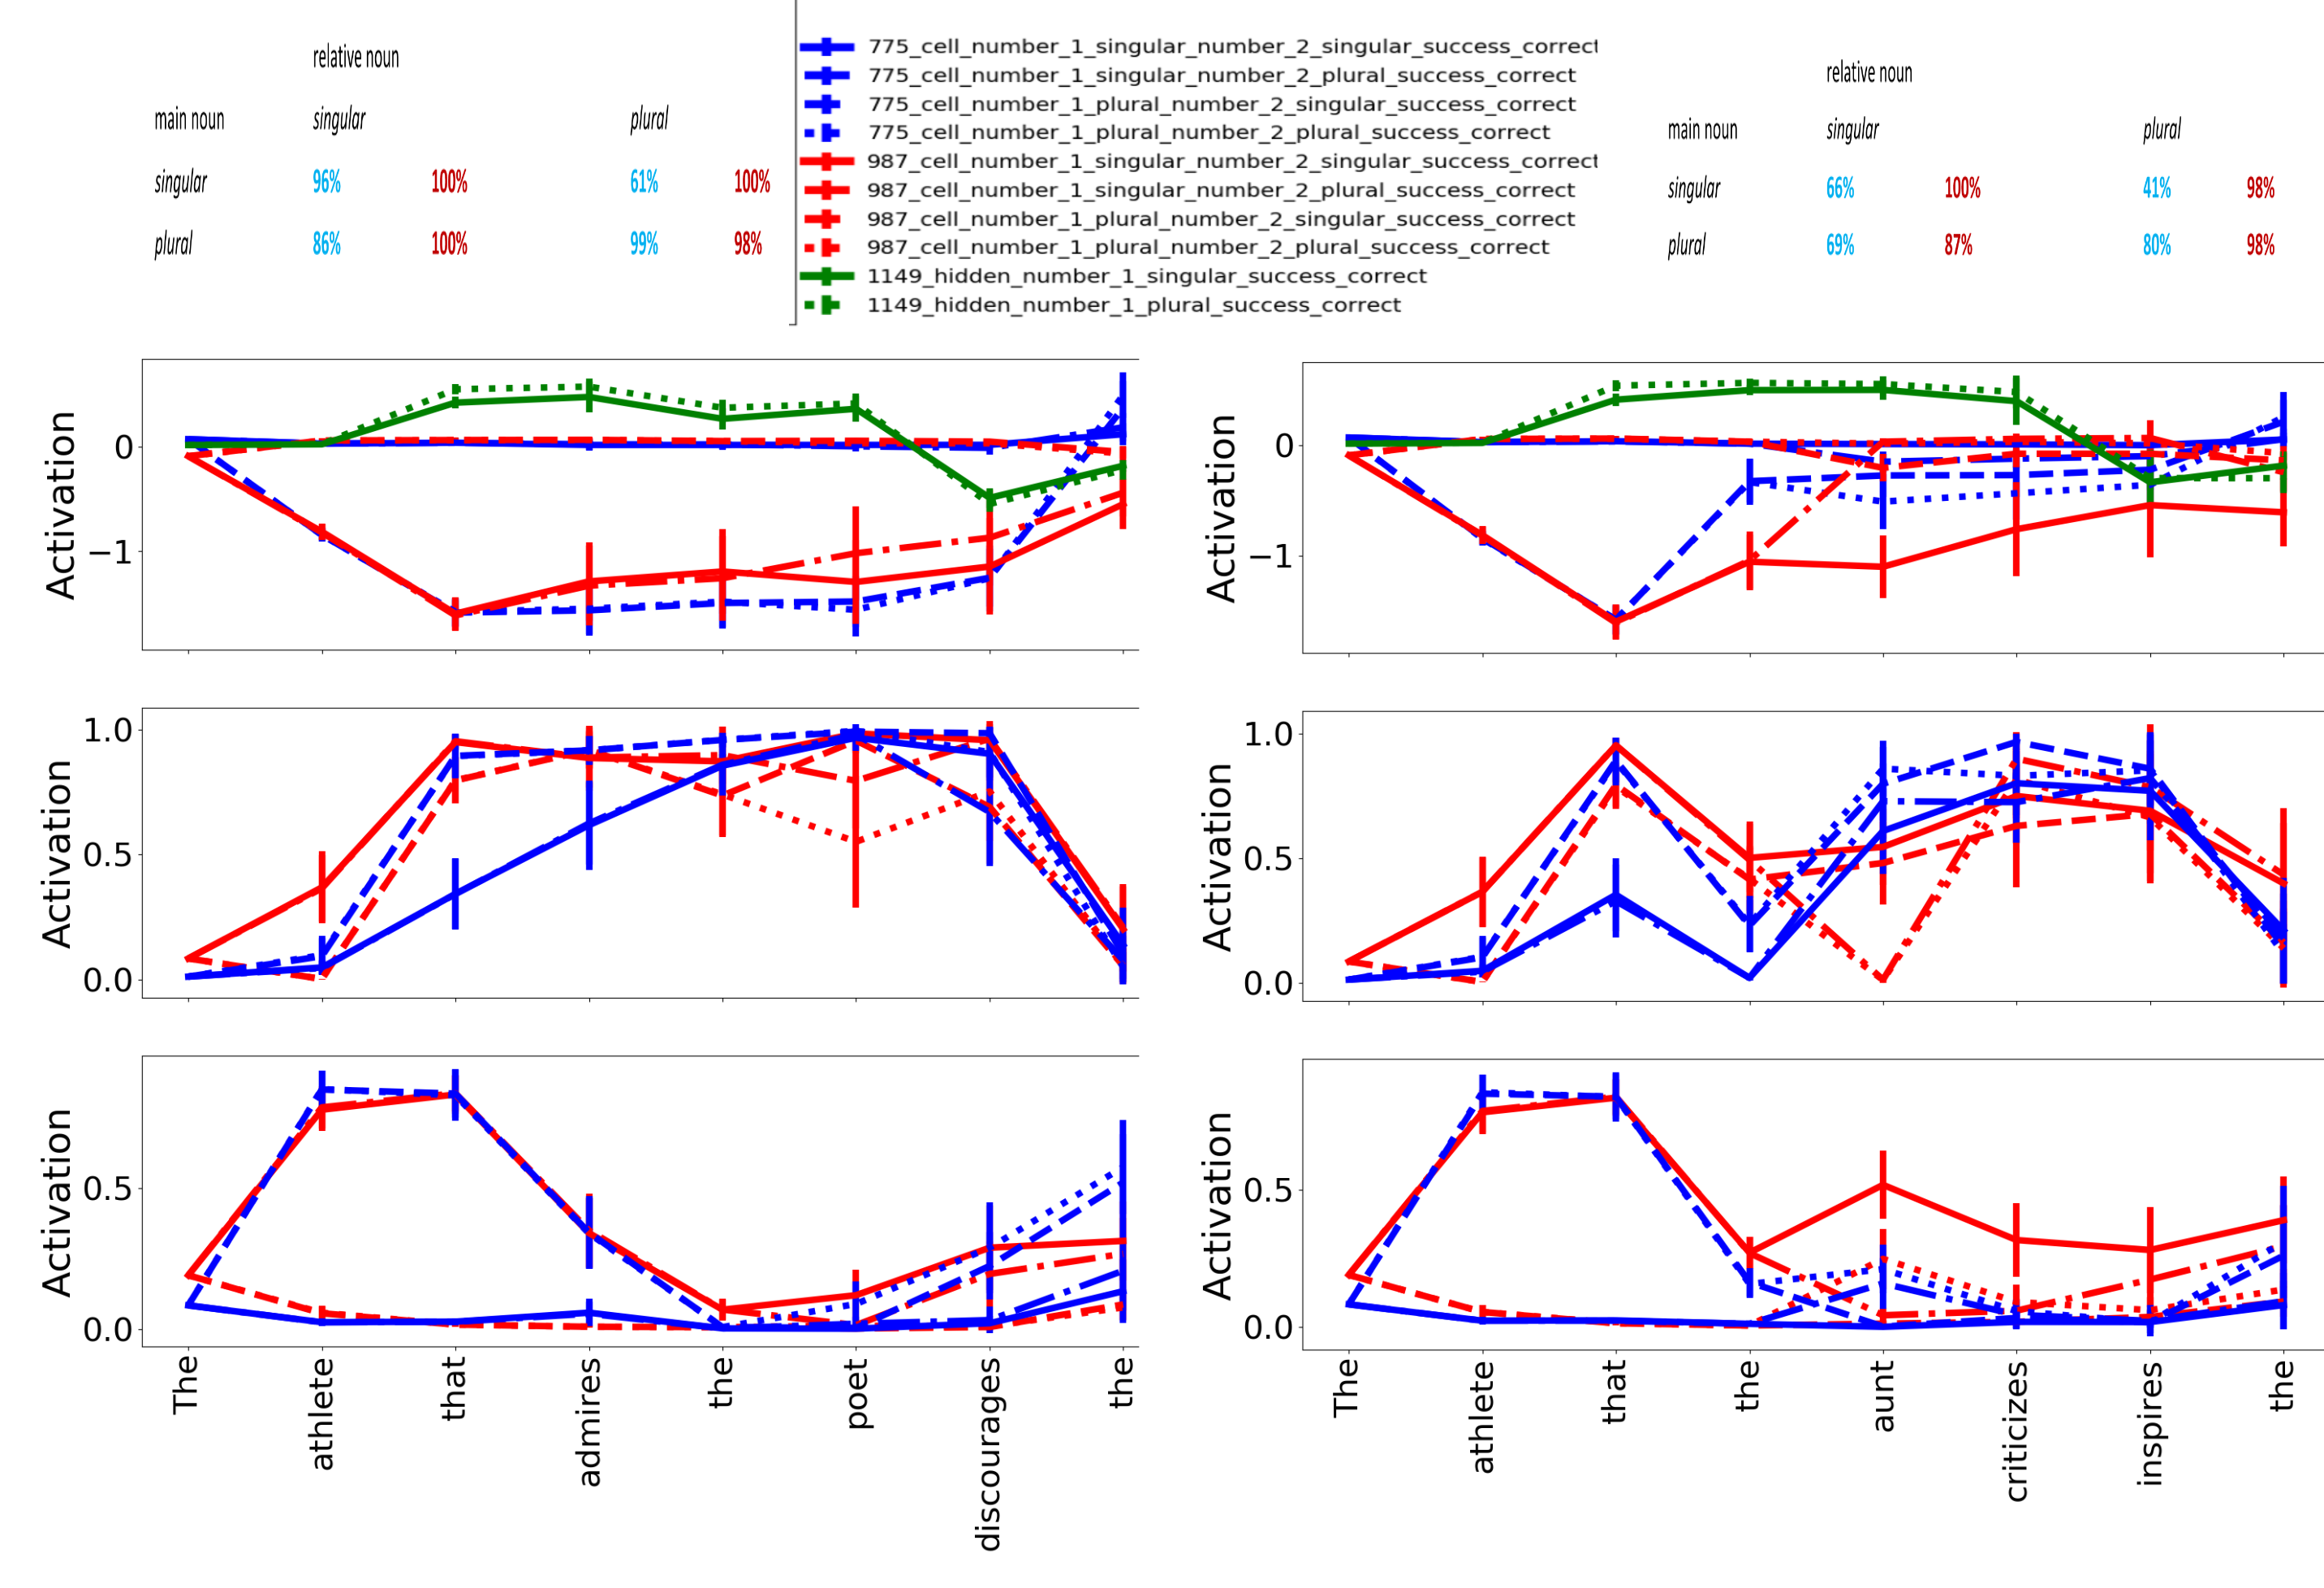
\includegraphics[width=\textwidth]{Figures/Figure8_RC.png}
\caption{Subject-verb agreement in relative clauses: agreement-task accuracy for (A) subject relatives and (B) object relatives. (C \& D) The corresponding cell activations for the number units (775 and 987) and the syntax unit 1149. (E \& F) The corresponding forget-gate activity and (G \& H) input-gate activity of the number units. }
\end{figure*}

\begin{figure}[b]
\centering
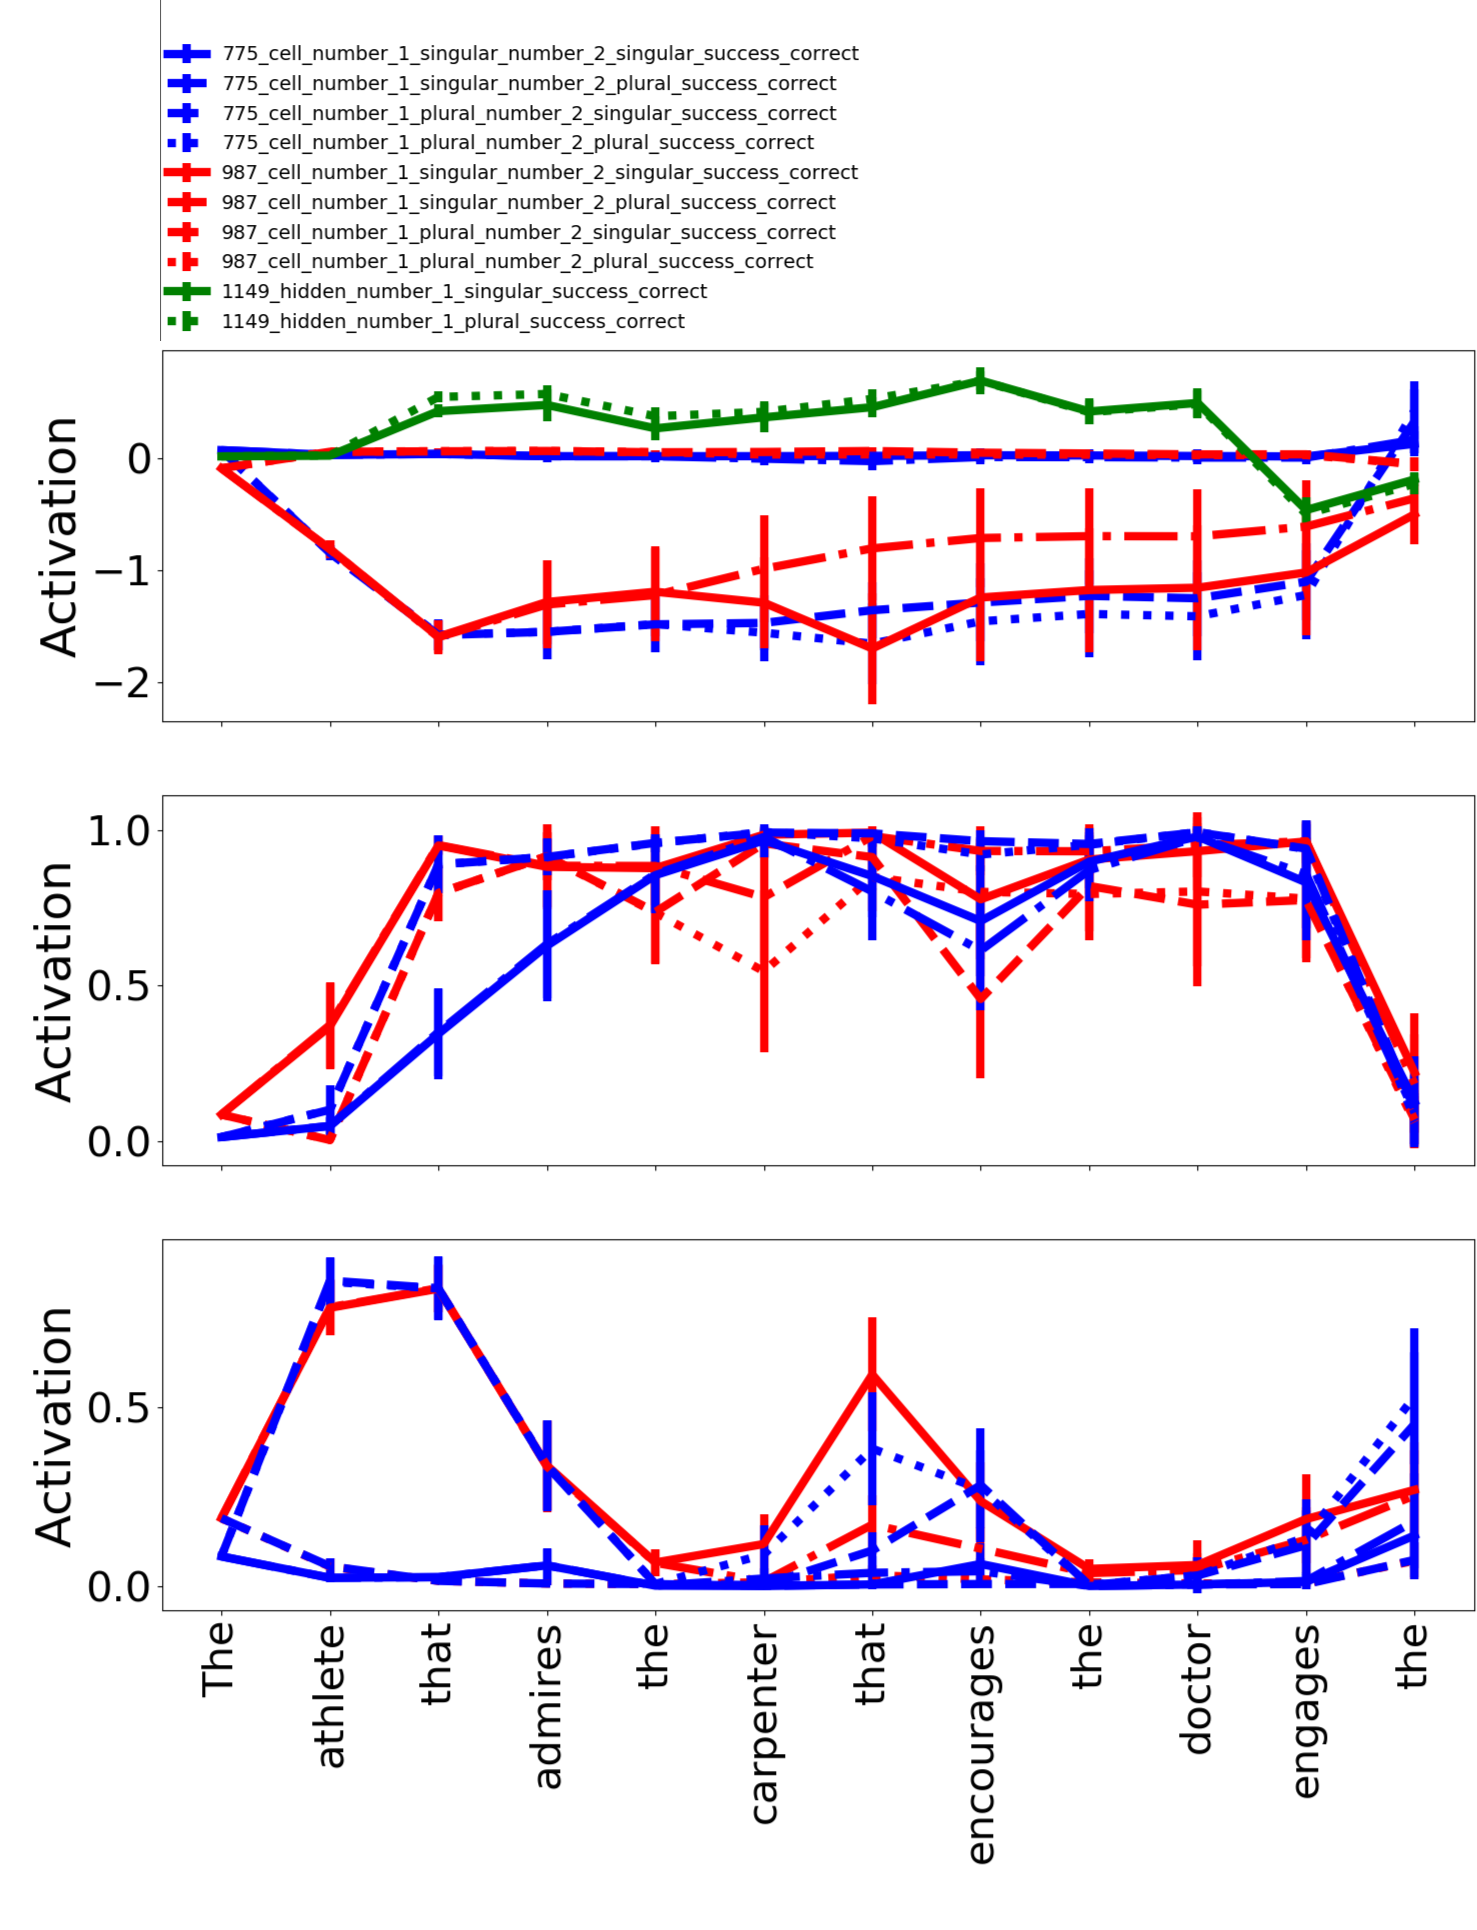
\includegraphics[width=\linewidth]{Figures/Figure9_doubleRC.png}
\caption{Processing of subject relatives with double embeddings. (A) Cell activity of the number and syntax units (775, 987 and 1149) (B) The corresponding forget-gate and (C) input-gate activity.}
\end{figure}

Sentences with relative clauses (RCs) and their processing are of major interset in linguistic and psycholinguistic (cite) given that they involve embedding, syntactic movement (object relatives)...and require theoretical...\textcolor{red}{complete this introductory sentence about RCs}. This section explores the dynamics of the LR-number units and syntax unit 1150 during the processing of sentences with RCs. Specifically, we looked into number agreement during the processing of subject and object relatives, the latter of which is known to be more prone for errors in humans (cite). In particular, we analyzed the performance of the network on the NA-task and compared it to the underlying gate dynamics of the LR-number units, similarly to the nounPP case in section 5.1. 

Figure X shows the behavioral results of the network on the subjrel (panel A) and objrel (panel B) NA-tasks. Network performance on the subjrel NA-task was relatively high compared to the objrel task, in both the congruent (main diagonal) and incongruent cases (off-diagonal values) \textcolor{red}{requires quantification}. This matches human performance on similar tasks (cite) and extends the analysis of previously reported results on the processing of RCs by LSTM-LM (Linzen 2018). Interestingly, when the subject is singular, more errors are made by human participants compared to the plural case (Bock). This matches LSTM-LM performance in both subjrel and objrel tasks and in both congurent and incongruent cases: $ACC^subjrel_{SS}<ACC^subjrel_{SP}, ACC^subjrel_{SP}<ACC^subjrel_{PS}, ACC^objrel{SS}<ACC^objrel{SP}, ACC^objrel{SP}<ACC^objrel{PS}$. Given that the language model was trained on word tokens, these results suggest that the source for the singular-plural assymetry resides at the word-level statistics in the corpus and not at the segmental level (cite Miller and Bock), also for humans.

and the corresponding gate dynamics during the processing of the sentences (panels C and D, respectively).


To explore thduring the processing of sentences with two embedded subject-relatuve clauses (double-subjrel). 

% 
% Discussion

\section{Discussion}
More generally, we provided the most detailed analysis of the inner
dynamics of an LSTM performing a linguistic task we are aware of. We
think that similar studies should complement currently popular
black-box tests, to achieve a true understanding of language
processing in neural networks. \textbf{Here, we might want to mention
  the need for future work on relative clauses, as well as on other
  models, such as transformers.}

From a more cognitive perspective, we hope our granular
understanding of how LSTMs perform number agreement will inform work
on computational modeling of neural sentence processing data, as we
conjecture a similar interaction between syntactic and
feature-carrying units might be implemented in the human
brain. Intriguingly, we observed differential handling of singular and
plural information, with the latter being more reliably processed,
resulting in more robust plural agreement. As a similar asymmetry has
also been observed in humans (\textbf{REFS}), one exciting avenue for
future work might consist in looking for different singular/plural
processing networks in the human brain.


% Acknowledgments
% \section*{Acknowledgments}
% \lipsum[1]

\bibliography{marco}
\bibliographystyle{naaclhlt2016}


\end{document}

